\section{Results}\label{sec:results}

% Every table below is generated by evaluation/tables.py and every figure by evaluation/figures.py. Numbers in the
% prose come from evaluation/analysis/report.md (stats.py) and evaluation/analysis/robust_report.md (robust.py),
% final run of 205 configurations. The statistical tests behind each statement are in Appendix B.

This section reports the main results for each research question. The statistical tests behind each statement are in Appendix~\ref{app:stats}. Qwen has no configurations for Grafana and Online Boutique, because their prompts exceeded its provider's request limit (Section~\ref{sec:threats}), so it contributes 30 configurations instead of 42.

\subsection{RQ1: LLM-generated versus human-written configurations}\label{sec:res-rq1}

Table~\ref{tab:overview-neutral} and Figure~\ref{fig:dimensions-neutral} compare each model's neutral-prompt configurations with the manifests the projects ship. Five of the seven human manifests are demonstration manifests (Table~\ref{tab:dataset}). So this is a comparison with what the projects ship, not with production practice. With only seven human manifests, it can also show only large differences.

% generated by evaluation/tables.py -- do not edit
\begin{table*}[t]
\centering\small
\caption{Six-dimension results, neutral prompt. Binary rows: percentage (count/n); continuous rows: median [interquartile range]. The human column is the shipped manifest of each project (one per project). Continuous rows are computed over the configurations for which the metric is defined: static scores over parsed configurations, D5 time to Ready and D6 over deployed ones, so their n can be smaller than the column total. D6 downtime depends mainly on the replica count of the faulted workload (Section~\ref{sec:res-rq5}).}\label{tab:overview-neutral}
\begin{tabular}{lrrrrrr}
\toprule
Metric & Human & Claude & DeepSeek & Gemini & GPT & Qwen \\ \midrule
Configurations & 7 & 21 & 21 & 21 & 21 & 15 \\ \midrule
D1 all objects API-accepted & 100 (7/7) & 100 (21/21) & 100 (21/21) & 90 (19/21) & 100 (21/21) & 67 (10/15) \\
D2 passes PSS baseline & 100 (7/7) & 86 (18/21) & 86 (18/21) & 84 (16/19) & 90 (19/21) & 100 (14/14) \\
D2 passes PSS restricted & 0 (0/7) & 10 (2/21) & 5 (1/21) & 0 (0/19) & 24 (5/21) & 7 (1/14) \\
D2 secret check flags a credential & 43 (3/7) & 52 (11/21) & 52 (11/21) & 53 (10/19) & 57 (12/21) & 64 (9/14) \\
D5 fully Ready & 100 (7/7) & 86 (18/21) & 67 (14/21) & 71 (15/21) & 76 (16/21) & 60 (9/15) \\
D5 smoke test passes & 86 (6/7) & 90 (19/21) & 76 (16/21) & 86 (18/21) & 76 (16/21) & 47 (7/15) \\
\midrule
D2 Kubescape compliance (\%) & 75.0 & 76.7 & 76.7 & 76.7 & 79.8 & 70.0 \\[-2pt]
 & {\scriptsize[73.0, 76.6]} & {\scriptsize[76.4, 78.1]} & {\scriptsize[71.7, 80.6]} & {\scriptsize[72.4, 80.0]} & {\scriptsize[76.7, 82.2]} & {\scriptsize[70.0, 73.1]} \\ \addlinespace[3pt]
D2 Trivy high+critical findings & 9.0 & 12.0 & 10.0 & 12.0 & 12.0 & 12.0 \\[-2pt]
 & {\scriptsize[1.0, 13.5]} & {\scriptsize[2.0, 17.0]} & {\scriptsize[2.0, 15.0]} & {\scriptsize[1.5, 15.0]} & {\scriptsize[4.0, 23.0]} & {\scriptsize[10.2, 15.8]} \\ \addlinespace[3pt]
D3 Polaris score & 62.0 & 67.0 & 67.0 & 65.0 & 69.0 & 58.5 \\[-2pt]
 & {\scriptsize[58.5, 72.5]} & {\scriptsize[66.0, 73.0]} & {\scriptsize[61.0, 77.0]} & {\scriptsize[59.5, 71.0]} & {\scriptsize[67.0, 73.0]} & {\scriptsize[56.0, 63.5]} \\ \addlinespace[3pt]
D3 reliability checklist (\%) & 30.7 & 50.0 & 44.9 & 40.0 & 54.0 & 24.5 \\[-2pt]
 & {\scriptsize[20.0, 40.0]} & {\scriptsize[40.0, 53.1]} & {\scriptsize[23.3, 55.0]} & {\scriptsize[18.6, 55.1]} & {\scriptsize[50.0, 56.7]} & {\scriptsize[17.5, 30.0]} \\ \addlinespace[3pt]
D3 smells per KLOC & 36.0 & 31.7 & 33.6 & 39.0 & 19.2 & 69.0 \\[-2pt]
 & {\scriptsize[23.1, 47.5]} & {\scriptsize[16.3, 36.4]} & {\scriptsize[6.9, 50.8]} & {\scriptsize[11.8, 54.5]} & {\scriptsize[7.1, 36.0]} & {\scriptsize[25.0, 74.3]} \\ \addlinespace[3pt]
D4 requirements met (\%) & 100.0 & 100.0 & 96.3 & 96.3 & 100.0 & 100.0 \\[-2pt]
 & {\scriptsize[95.8, 100.0]} & {\scriptsize[92.3, 100.0]} & {\scriptsize[91.7, 100.0]} & {\scriptsize[91.7, 100.0]} & {\scriptsize[100.0, 100.0]} & {\scriptsize[93.3, 100.0]} \\ \addlinespace[3pt]
D5 time to Ready (s) & 20.1 & 32.7 & 18.8 & 20.5 & 31.2 & 16.8 \\[-2pt]
 & {\scriptsize[14.6, 64.0]} & {\scriptsize[15.8, 37.6]} & {\scriptsize[16.6, 35.7]} & {\scriptsize[11.1, 40.1]} & {\scriptsize[19.9, 43.2]} & {\scriptsize[12.0, 26.2]} \\ \addlinespace[3pt]
D6 recovery time (s) & 7.8 & 16.1 & 16.2 & 14.2 & 16.7 & 12.8 \\[-2pt]
 & {\scriptsize[6.9, 26.2]} & {\scriptsize[9.7, 27.2]} & {\scriptsize[12.9, 20.8]} & {\scriptsize[7.5, 17.2]} & {\scriptsize[13.7, 18.3]} & {\scriptsize[8.4, 17.1]} \\ \addlinespace[3pt]
D6 downtime per fault (s) & 6.2 & 6.5 & 5.3 & 5.6 & 6.6 & 5.3 \\[-2pt]
 & {\scriptsize[2.8, 8.4]} & {\scriptsize[2.4, 7.3]} & {\scriptsize[4.5, 7.2]} & {\scriptsize[3.4, 7.0]} & {\scriptsize[3.7, 7.4]} & {\scriptsize[3.1, 6.3]} \\ \addlinespace[3pt]
\bottomrule
\end{tabular}
\end{table*}


\begin{figure*}[t]
\centering
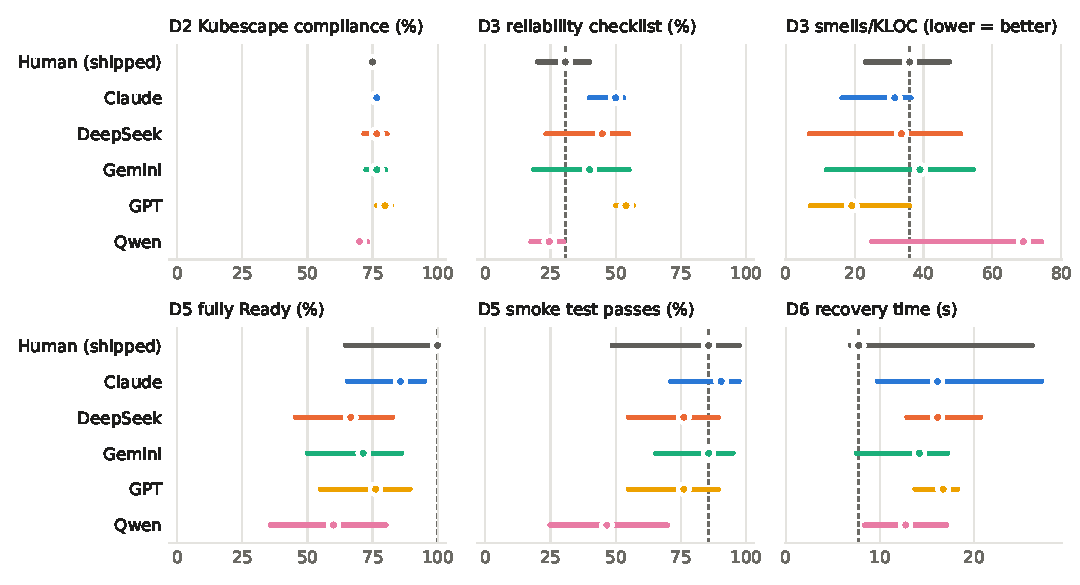
\includegraphics[width=\textwidth]{figures/fig_dimensions_neutral.pdf}
\caption{Neutral-prompt results per source. Dots show medians (continuous metrics) or proportions (binary metrics). Bars show interquartile ranges or 95\% Wilson intervals. The dashed line marks the human manifests. D1 and D4 are omitted because every source's median is 96--100\%. Human: $n=7$; Claude, DeepSeek, Gemini, GPT: $n=21$; Qwen: $n=15$; D6 is conditional on deployment.}
\label{fig:dimensions-neutral}
\end{figure*}

\textbf{Correctness (D1).} The API server accepted every object of every human manifest and of every neutral-prompt configuration from Claude, DeepSeek and GPT. Two of Gemini's 21 configurations, both for the Kubernetes Dashboard, are missing, because the provider withheld them for reproducing training data too closely. Qwen had every object accepted in only 10 of its 15 configurations. It mostly declared Services with several unnamed ports, which a schema validator accepts but the API server rejects.

\textbf{Security (D2).} The static security of the generated configurations is close to that of the shipped manifests. Median Kubescape compliance is 75.0\% for the human manifests, 76.7\% for Claude, DeepSeek and Gemini, 79.8\% for GPT and 70.0\% for Qwen. For every model, the project-level difference from the human manifests is within about ten points. This excludes large differences but not moderate ones. Few configurations reach the \texttt{restricted} Pod Security Standard (none of the human manifests; 0--24\% per model), while 84--100\% of every source passes \texttt{baseline}. The secret check flags 43\% of the human manifests and 52--64\% of each model's configurations, with no significant difference.

\textbf{Static reliability (D3).} Claude and GPT cover more of the reliability checklist than the shipped manifests (medians 50.0\% and 54.0\% against 30.7\%). This difference also holds at project level. Gemini (40.0\%), DeepSeek (44.9\%) and Qwen (24.5\%) are close to the human level.

\textbf{Requirements (D4).} Requirement satisfaction is high for every source (medians 96--100\%).

\textbf{Deployment (D5) and recovery (D6).} The models' configurations became fully Ready in 60\% (Qwen) to 86\% (Claude) of cases, and passed the smoke test in 47\% (Qwen) to 90\% (Claude). All seven human manifests became fully Ready, and six passed their smoke test. The exception, Sock Shop, became Ready, but its cart service failed: an image tag that the manifest leaves unpinned now resolves to an incompatible database release. We selected projects only if their human manifest could be deployed (Section~\ref{sec:method-dataset}). So the human rates are a reference, not a test. Every configuration that reached fault injection recovered from every fault, except one GPT configuration. Recovery took 7.8~s (median) for the human manifests and 13--17~s per model, a difference that is not significant.

In short, under the neutral prompt the models match the shipped manifests on static security, GPT and Claude cover more of the reliability checklist, and Qwen is lower on every static score.

\subsection{RQ2: Most frequent misconfigurations}\label{sec:res-rq2}

Table~\ref{tab:rahman} reports, for each source and prompt, the share of configurations showing each security misconfiguration category of \citet{rahman2023k8smisconfig}.

% generated by evaluation/tables.py -- do not edit
\begin{table*}[t]
\centering\small
\caption{Share of configurations (\%) exhibiting each security misconfiguration category of Rahman et al., detected with the rules of their SLI-KUBE tool. N = neutral prompt, P = production prompt. No configuration from any source exhibits activation of hostIPC, activation of hostNetwork, activation of hostPID, capability misuse, escalated privileges for child processes, privileged securityContext. Following SLI-KUBE, a hard-coded secret is any literal value under a key naming a user, password, token or secret. The D2 secret check of Table~\ref{tab:overview-neutral} is stricter (user names and placeholder values such as \texttt{changeme} are not counted, known credential token formats are), so its rates are lower.}\label{tab:rahman}
\resizebox{\textwidth}{!}{%
\begin{tabular}{lrrrrrrrrrrr}
\toprule
Category & Human & Claude N & Claude P & DeepSeek N & DeepSeek P & Gemini N & Gemini P & GPT N & GPT P & Qwen N & Qwen P \\ \midrule
Absent resource limit & 100 & 57 & 0 & 48 & 10 & 47 & 16 & 24 & 5 & 79 & 33 \\
Absent securityContext & 71 & 76 & 0 & 76 & 25 & 79 & 63 & 76 & 14 & 86 & 75 \\
Docker socket mounting & 0 & 14 & 0 & 14 & 5 & 16 & 16 & 10 & 0 & 7 & 0 \\
Hard-coded secret & 57 & 67 & 67 & 67 & 70 & 68 & 68 & 71 & 71 & 64 & 67 \\
Insecure HTTP & 0 & 14 & 14 & 14 & 10 & 16 & 16 & 14 & 14 & 21 & 25 \\
\bottomrule
\end{tabular}}
\end{table*}


Three categories dominate for every source:
\begin{itemize}
\item A hard-coded secret, by the SLI-KUBE rule, appears in 57\% of the human manifests and 64--71\% of each model's configurations under both prompts. The production prompt does not reduce it.
\item An absent security context appears in 71\% of the human manifests and 76--86\% of neutral-prompt configurations.
\item An absent resource limit appears in every human manifest and 24--79\% of neutral-prompt configurations.
\end{itemize}
For Claude, DeepSeek and GPT, the production prompt removes most of the last two (for Claude, from 57\% and 76\% to 0\%). Gemini and Qwen keep an absent security context in most configurations (63\% and 75\%). Docker socket mounting (7--16\% of neutral configurations) occurs only for Sock Shop: its Compose file mounts the socket, while its human manifest does not (Section~\ref{sec:disc-compose}).

Reliability settings are missing in a similar way (Appendix~\ref{app:stats}, Table~\ref{tab:checklist-items}). Under the neutral prompt, nearly every workload of every source, human manifests included, runs a single replica without a PodDisruptionBudget, anti-affinity or an explicit rolling-update strategy, and 35--68\% lack readiness and liveness probes. The production prompt adds these settings mainly for Claude and GPT (for Claude, single-replica workloads fall from 98\% to 23\%), partly for DeepSeek, and hardly at all for Gemini and Qwen.

\subsection{RQ3: Differences between models and consistency}\label{sec:res-rq3}

The models differ clearly in their static scores. GPT and Claude score highest, and Qwen and Gemini lowest, on Kubescape compliance, checklist coverage and Polaris score. Under the production prompt, the gap is larger: Claude, GPT and DeepSeek score higher than Gemini and Qwen on all three. Deployment success, however, does not differ significantly between models once the differences between projects are taken into account. These are comparisons of model-and-access configurations (Section~\ref{sec:method-generation}), not of models in isolation.

Gemini is the most consistent model: its three samples of a project usually receive the same Kubescape compliance and checklist coverage. Qwen is the least consistent. Whether a configuration works is less repeatable than its static scores. The three samples agree on becoming fully Ready in 86\% of cells for Claude, 71\% for Gemini, 50\% for GPT and Qwen and 43\% for DeepSeek, and on the smoke-test outcome in 64--71\% of cells for every model.

\subsection{RQ4: Why configurations fail at runtime, and whether static analysis predicts it}\label{sec:res-rq4}

Figure~\ref{fig:attrition} follows every configuration through the pipeline. Of the 198 generated configurations, 184 were schema-valid and 180 had every object accepted. But only 128 became fully Ready, 136 passed their smoke test and 118 did both. Most of the loss happens at deployment, not at validation, and it is larger under the production prompt.

\begin{figure*}[t]
\centering
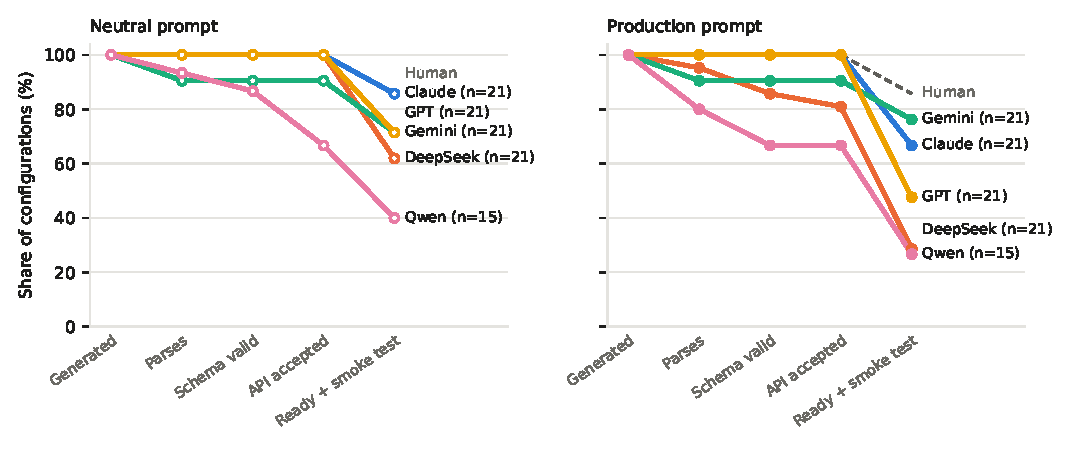
\includegraphics[width=\textwidth]{figures/fig_attrition.pdf}
\caption{Share of configurations surviving each stage, per model and prompt (open markers: neutral; filled: production). ``Ready + smoke'' is the share both fully Ready and passing the smoke test. Dashed line: the seven human manifests, which were selected for being deployable.}
\label{fig:attrition}
\end{figure*}

Being Ready and passing the smoke test are not the same. In 18 configurations, the application served every smoke-test request, but some workload never became Ready, most often an extra component copied from the Compose file, such as Sock Shop's load generator. In 10 others, every workload was Ready, but the application did not work, usually because a Service, RBAC object or NetworkPolicy on the request path was rejected or misdirected.

Table~\ref{tab:root-causes} gives the root cause of each of the 81 configurations (80 generated, one human) that were not both fully Ready and passing the smoke test. For 51, the cause is visible in the cluster's record; 22 are inferred, 5 are supported by a matched contrast and 3 remain undetermined. The most frequent causes are:
\begin{itemize}
\item host-level Compose services that fail while the application works (10);
\item invalid YAML or objects that the API server rejects (8);
\item hardening that stops a database (8);
\item liveness probes that kill slow-starting services (6).
\end{itemize}
The hardening and probe causes are concentrated under the production prompt (23 of their 30 failures).

% generated by evaluation/tables.py -- do not edit
\begin{table*}[t]
\centering\small
\caption{Root cause of every configuration that was not both fully Ready and passing its smoke test, by model and prompt (N = neutral, P = production). Obs.\ = cases whose mechanism is directly visible in the cluster's record (exit reason, log lines, events, rejected objects or provider stop reason); the remainder are inferred from the manifest together with the observed status, or, for two mechanisms, supported by a matched contrast.}\label{tab:root-causes}
\resizebox{\textwidth}{!}{%
\begin{tabular}{lrrrrrrrrr}
\toprule
Mechanism & Claude & DeepSeek & Gemini & GPT & Qwen & N & P & Human & Obs. \\ \midrule
\multicolumn{10}{l}{\textit{Hardening blocks the workload}} \\
\quad Capability drop or fixed UID stops the database & 3 & 3 & 0 & 2 & 0 & 0 & 8 & 0 & 3/8 \\
\quad runAsNonRoot on an image whose user cannot be verified & 0 & 1 & 0 & 2 & 0 & 1 & 2 & 0 & 0/3 \\
\quad Service-account token disabled for a component that needs the API & 0 & 0 & 0 & 1 & 0 & 0 & 1 & 0 & 1/1 \\
\quad NetworkPolicy blocks a documented internal route & 1 & 1 & 0 & 1 & 0 & 1 & 2 & 0 & 0/3 \\
\multicolumn{10}{l}{\textit{Probes and resource limits}} \\
\quad Liveness/startup probe kills a slow-starting service & 5 & 0 & 0 & 1 & 0 & 2 & 4 & 0 & 2/6 \\
\quad Memory limit too low (OOMKilled) & 0 & 1 & 0 & 1 & 0 & 1 & 1 & 0 & 2/2 \\
\quad Probe on the wrong port or path & 0 & 2 & 0 & 0 & 0 & 0 & 2 & 0 & 1/2 \\
\quad Probe calls a binary the image does not ship & 0 & 0 & 1 & 0 & 0 & 1 & 0 & 0 & 0/1 \\
\quad HTTP probe on a component without a server & 0 & 0 & 0 & 0 & 4 & 1 & 3 & 0 & 0/4 \\
\multicolumn{10}{l}{\textit{Compose file translated literally}} \\
\quad Host-level Compose services fail; application works & 1 & 2 & 6 & 1 & 0 & 7 & 3 & 0 & 10/10 \\
\multicolumn{10}{l}{\textit{Wrong values or references}} \\
\quad Service targets the wrong container port & 0 & 1 & 0 & 0 & 1 & 2 & 0 & 0 & 1/2 \\
\quad API server address overridden & 0 & 1 & 0 & 0 & 0 & 0 & 1 & 0 & 0/1 \\
\quad Volume references an undefined Secret & 0 & 1 & 0 & 0 & 0 & 1 & 0 & 0 & 1/1 \\
\quad RBAC does not allow updating the CSRF Secret & 0 & 0 & 0 & 1 & 3 & 2 & 2 & 0 & 0/4 \\
\quad No writable /tmp volume on a distroless image & 0 & 0 & 0 & 0 & 1 & 1 & 0 & 0 & 1/1 \\
\quad Image from a non-existent repository & 0 & 0 & 0 & 0 & 2 & 0 & 2 & 0 & 2/2 \\
\quad Required variable set to an empty value & 0 & 2 & 0 & 1 & 0 & 1 & 2 & 0 & 3/3 \\
\quad Non-existent command-line flag & 0 & 0 & 0 & 3 & 0 & 1 & 2 & 0 & 3/3 \\
\quad Placeholder domain enforced & 0 & 0 & 0 & 1 & 0 & 0 & 1 & 0 & 1/1 \\
\quad Points at a database host that does not exist & 0 & 1 & 0 & 1 & 0 & 1 & 1 & 0 & 2/2 \\
\quad TLS required by the client, not offered by the database & 0 & 1 & 0 & 0 & 0 & 0 & 1 & 0 & 1/1 \\
\multicolumn{10}{l}{\textit{Invalid or missing output}} \\
\quad Invalid YAML or object rejected by the API server & 0 & 1 & 0 & 0 & 7 & 4 & 4 & 0 & 8/8 \\
\quad RBAC object rejected (unquoted resource name) & 0 & 2 & 0 & 0 & 0 & 0 & 2 & 0 & 2/2 \\
\quad Reply ends before the YAML block closes & 0 & 0 & 1 & 0 & 2 & 1 & 2 & 0 & 3/3 \\
\quad Provider withheld the reply (recitation) & 0 & 0 & 3 & 0 & 0 & 2 & 1 & 0 & 3/3 \\
\multicolumn{10}{l}{\textit{Other}} \\
\quad Cause not determined & 0 & 2 & 0 & 1 & 0 & 2 & 1 & 0 & 0/3 \\
\quad Unpinned image tag drifted & 0 & 0 & 0 & 0 & 0 & 0 & 0 & 1 & 1/1 \\
\midrule
Total & 10 & 22 & 11 & 17 & 20 & 32 & 48 & 1 & 51/81 \\
\bottomrule
\end{tabular}}
\end{table*}


Higher static security and reliability scores show no positive association with deployment success (Figure~\ref{fig:static-runtime}). Configurations with higher scanner scores did not work more often, and this remains true when the prompt, the project and the model are taken into account (Appendix~\ref{app:stats}). Only requirement satisfaction is associated with success, and partly by construction: D4 checks that the documented components and settings are present, and without them a deployment cannot work.

\begin{figure*}[t]
\centering
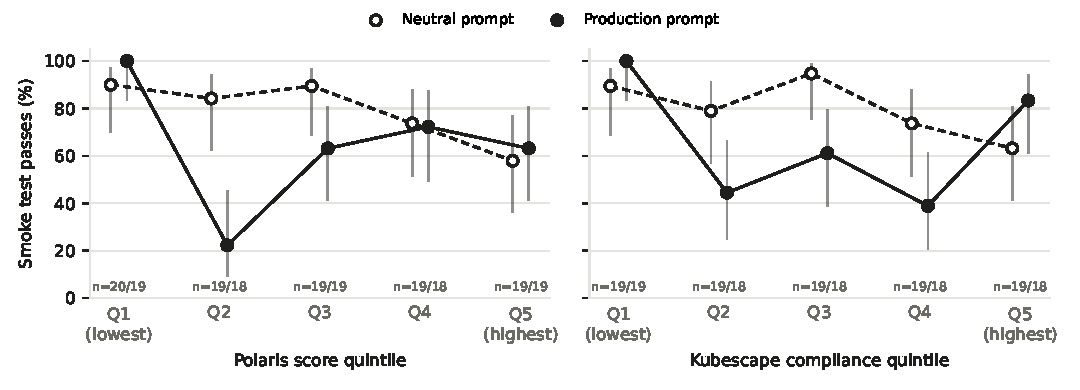
\includegraphics[width=\textwidth]{figures/fig_static_runtime.pdf}
\caption{Smoke-test pass rate by quintile of Polaris score (left) and Kubescape compliance (right), per prompt, with 95\% Wilson intervals. Neither score separates configurations that work from those that do not. $n$ = configurations per quintile (neutral/production); the adjusted analysis is in Appendix~\ref{app:stats}.}
\label{fig:static-runtime}
\end{figure*}

\subsection{RQ5: Effect of requesting production-ready output}\label{sec:res-rq5}

Figure~\ref{fig:tradeoff} summarises the effect for each model. Table~\ref{tab:overview-production} gives the production-prompt values.

% generated by evaluation/tables.py -- do not edit
\begin{table*}[t]
\centering\small
\caption{Six-dimension results, production prompt. Binary rows: percentage (count/n); continuous rows: median [interquartile range]. The human column is the shipped manifest of each project (one per project). Continuous rows are computed over the configurations for which the metric is defined: static scores over parsed configurations, D5 time to Ready and D6 over deployed ones, so their n can be smaller than the column total. D6 downtime depends mainly on the replica count of the faulted workload (Section~\ref{sec:res-rq5}).}\label{tab:overview-production}
\begin{tabular}{lrrrrrr}
\toprule
Metric & Human & Claude & DeepSeek & Gemini & GPT & Qwen \\ \midrule
Configurations & 7 & 21 & 21 & 21 & 21 & 15 \\ \midrule
D1 all objects API-accepted & 100 (7/7) & 100 (21/21) & 81 (17/21) & 90 (19/21) & 100 (21/21) & 67 (10/15) \\
D2 passes PSS baseline & 100 (7/7) & 100 (21/21) & 95 (19/20) & 84 (16/19) & 100 (21/21) & 100 (12/12) \\
D2 passes PSS restricted & 0 (0/7) & 62 (13/21) & 40 (8/20) & 16 (3/19) & 57 (12/21) & 0 (0/12) \\
D2 secret check flags a credential & 43 (3/7) & 57 (12/21) & 55 (11/20) & 58 (11/19) & 57 (12/21) & 67 (8/12) \\
D5 fully Ready & 100 (7/7) & 71 (15/21) & 43 (9/21) & 76 (16/21) & 57 (12/21) & 27 (4/15) \\
D5 smoke test passes & 86 (6/7) & 67 (14/21) & 38 (8/21) & 90 (19/21) & 57 (12/21) & 47 (7/15) \\
\midrule
D2 Kubescape compliance (\%) & 75.0 & 96.4 & 87.3 & 76.7 & 92.5 & 76.7 \\[-2pt]
 & {\scriptsize[73.0, 76.6]} & {\scriptsize[91.7, 100.0]} & {\scriptsize[84.1, 92.9]} & {\scriptsize[76.7, 84.3]} & {\scriptsize[89.8, 96.7]} & {\scriptsize[75.0, 79.7]} \\ \addlinespace[3pt]
D2 Trivy high+critical findings & 9.0 & 0.0 & 3.5 & 12.0 & 0.0 & 10.0 \\[-2pt]
 & {\scriptsize[1.0, 13.5]} & {\scriptsize[0.0, 4.0]} & {\scriptsize[1.0, 8.0]} & {\scriptsize[1.0, 15.0]} & {\scriptsize[0.0, 5.0]} & {\scriptsize[5.0, 12.8]} \\ \addlinespace[3pt]
D3 Polaris score & 62.0 & 90.0 & 85.0 & 71.0 & 86.0 & 69.5 \\[-2pt]
 & {\scriptsize[58.5, 72.5]} & {\scriptsize[86.0, 91.0]} & {\scriptsize[81.0, 87.5]} & {\scriptsize[68.0, 82.5]} & {\scriptsize[84.0, 89.0]} & {\scriptsize[65.2, 75.0]} \\ \addlinespace[3pt]
D3 reliability checklist (\%) & 30.7 & 80.7 & 64.0 & 55.2 & 75.0 & 41.2 \\[-2pt]
 & {\scriptsize[20.0, 40.0]} & {\scriptsize[70.0, 85.0]} & {\scriptsize[58.9, 79.2]} & {\scriptsize[52.5, 60.0]} & {\scriptsize[69.0, 79.0]} & {\scriptsize[30.0, 54.2]} \\ \addlinespace[3pt]
D3 smells per KLOC & 36.0 & 8.1 & 10.7 & 27.4 & 7.1 & 26.6 \\[-2pt]
 & {\scriptsize[23.1, 47.5]} & {\scriptsize[3.5, 10.4]} & {\scriptsize[1.7, 17.5]} & {\scriptsize[5.8, 43.2]} & {\scriptsize[0.0, 11.0]} & {\scriptsize[10.7, 42.7]} \\ \addlinespace[3pt]
D4 requirements met (\%) & 100.0 & 100.0 & 100.0 & 92.3 & 96.3 & 98.2 \\[-2pt]
 & {\scriptsize[95.8, 100.0]} & {\scriptsize[91.7, 100.0]} & {\scriptsize[93.7, 100.0]} & {\scriptsize[88.7, 98.2]} & {\scriptsize[91.7, 100.0]} & {\scriptsize[92.3, 100.0]} \\ \addlinespace[3pt]
D5 time to Ready (s) & 20.1 & 33.0 & 27.5 & 18.2 & 24.9 & 23.0 \\[-2pt]
 & {\scriptsize[14.6, 64.0]} & {\scriptsize[22.5, 42.8]} & {\scriptsize[16.6, 39.8]} & {\scriptsize[14.3, 35.0]} & {\scriptsize[18.6, 46.5]} & {\scriptsize[15.8, 32.5]} \\ \addlinespace[3pt]
D6 recovery time (s) & 7.8 & 15.0 & 14.6 & 13.7 & 9.2 & 17.1 \\[-2pt]
 & {\scriptsize[6.9, 26.2]} & {\scriptsize[10.9, 21.4]} & {\scriptsize[12.4, 22.7]} & {\scriptsize[8.5, 17.4]} & {\scriptsize[5.9, 17.9]} & {\scriptsize[15.6, 22.8]} \\ \addlinespace[3pt]
D6 downtime per fault (s) & 6.2 & 0.3 & 0.2 & 5.5 & 0.3 & 6.9 \\[-2pt]
 & {\scriptsize[2.8, 8.4]} & {\scriptsize[0.1, 6.0]} & {\scriptsize[0.2, 3.9]} & {\scriptsize[0.2, 7.0]} & {\scriptsize[0.2, 6.9]} & {\scriptsize[3.3, 8.4]} \\ \addlinespace[3pt]
\bottomrule
\end{tabular}
\end{table*}


\textbf{Static scores go up.} For the median model--project pair, the production prompt adds 9.1 points of Kubescape compliance, 22.5 points of checklist coverage and 13.3 points of Polaris score, and removes 3.5 high or critical Trivy findings and 16.9 smells per thousand lines. The gain is largest for Claude (Kubescape $+19.8$ points), then GPT ($+12.4$) and DeepSeek ($+10.1$), and small for Qwen ($+5.7$) and Gemini ($+3.6$). In addition, 27 configurations pass the \texttt{restricted} Pod Security Standard only under the production prompt, and one only under the neutral one.

\textbf{Deployment success goes down.} The smoke-test pass rate falls from 76.8\% (76 of 99) to 60.6\% (60 of 99), and the fully Ready rate from 72.7\% to 56.6\%. Across model--project pairs, the fully Ready rate falls in 13 and rises in 3, and the smoke-test rate falls in 12 and rises in 3; both declines are significant. Gemini is the exception: its rates are nearly the same under both prompts (Figure~\ref{fig:tradeoff}), and its scores also changed least. The added failures are those of Section~\ref{sec:res-rq4}: hardening that stops a database and liveness probes that kill slow-starting services.

% Full-width float: a one-column float queues behind the earlier full-width figure, and an inline one leaves gaps
\begin{figure*}[t]
\centering
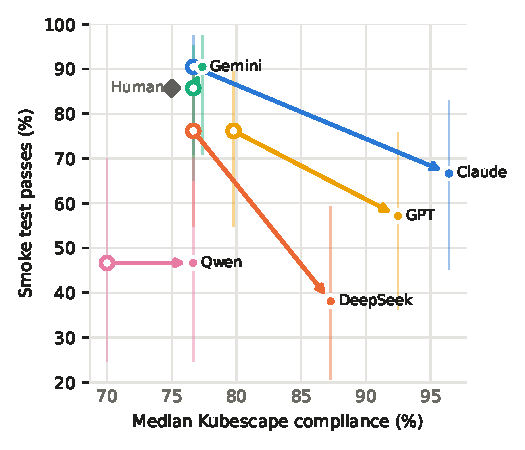
\includegraphics[width=0.55\textwidth]{figures/fig_tradeoff.pdf}
\caption{Static security against deployment success, per model. Open marker = neutral prompt, filled = production prompt (vertical bars: 95\% Wilson intervals of the smoke-test rate); diamond = human manifests. Two coincident markers (Claude neutral, Gemini production) are offset slightly.}
\label{fig:tradeoff}
\end{figure*}

\textbf{Recovery does not change.} Every configuration that recovered from all faults under one prompt also did under the other. Downtime during a fault depends almost entirely on the number of replicas: about 6--7~s with one replica, for every source, and 0.2~s with two or more. The production prompt gives the faulted workload two or more replicas in 55\% of configurations, against 12\% under the neutral prompt and none of the human manifests.
